% ============================================================
%  SOS/A FORMELSAMMLUNG — Teil 0
%  Mathematische Grundlagen | Determinanten & Eigenwerte
% ============================================================

\bereich[cKap0]{Teil 0: Mathematische Grundlagen}

\begin{formelreihe}
  \formelblock{Determinante $2\times2$}{
    \det\!\begin{bsmallmatrix}a&b\\c&d\end{bsmallmatrix}=ad-bc} &
  \parbox[t]{\linewidth}{%
  {\scriptsize\scshape\color{gray!65!black} Determinante $3\times3$ (Sarrus)}\\[0.03em]
  \begin{minipage}[c]{0.62\linewidth}\footnotesize
    $\displaystyle\begin{aligned}
      &\det\!\begin{bsmallmatrix}a&b&c\\d&e&f\\g&h&i\end{bsmallmatrix}\\
      &=a(ei\!-\!fh)-b(di\!-\!fg)\\
      &\quad+\,c(dh\!-\!eg)
    \end{aligned}$
  \end{minipage}\hfill
  \begin{minipage}[c]{0.34\linewidth}\centering
  % Sarrus-Schema grafisch: 1.\&2. Spalte anh\"angen, Diagonalprodukte
  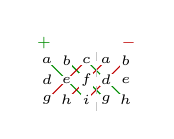
\begin{tikzpicture}[x=2.5mm,y=2.5mm,line width=0.4pt,font=\tiny,baseline=(current bounding box.center)]
    \begin{scope}[line cap=round]
      \draw[green!55!black] (0,2)--(2,0);
      \draw[green!55!black] (1,2)--(3,0);
      \draw[green!55!black] (2,2)--(4,0);
      \draw[red!75!black]   (0,0)--(2,2);
      \draw[red!75!black]   (1,0)--(3,2);
      \draw[red!75!black]   (2,0)--(4,2);
    \end{scope}
    \draw[gray!45,dashed] (2.5,-0.55)--(2.5,2.55);
    \foreach \x/\y/\l in {0/2/a,1/2/b,2/2/c,3/2/a,4/2/b,%
                          0/1/d,1/1/e,2/1/f,3/1/d,4/1/e,%
                          0/0/g,1/0/h,2/0/i,3/0/g,4/0/h}
      \node[fill=white,inner sep=0.5pt] at (\x,\y) {$\l$};
    \node[green!55!black] at (-0.15,2.9) {$\scriptscriptstyle+$};
    \node[red!75!black]   at ( 4.15,2.9) {$\scriptscriptstyle-$};
  \end{tikzpicture}
  \end{minipage}} &
  \beispielblock{Determinante}{\begin{aligned}
    &\det\!\begin{bsmallmatrix}1&2&0\\0&3&1\\1&0&2\end{bsmallmatrix}\\
    &=1(6\!-\!0)-2(0\!-\!1)+0\\
    &=6+2=8
  \end{aligned}} \\[0.3em]

  \formelblock{Eigenwerte $\lambda_i$}{\begin{aligned}
    &\det(\lambda\mathbf{I}-\mathbf{A})=0\\
    &\text{(charakterist. Polynom)}\\[0.12em]
    &\lambda\mathbf{I}-\mathbf{A}=
      \begin{bsmallmatrix}\lambda-a&-b\\-c&\lambda-d\end{bsmallmatrix}\\
    &{\scriptstyle\lambda\text{ nur auf der Diagonale!}}\\[0.12em]
    &\mathbf{A}\,\mathbf{v}_i=\lambda_i\,\mathbf{v}_i
  \end{aligned}} &
  \parbox[t]{\linewidth}{%
    \formelblock{$2\times2$-Schnellformel}{%
      \lambda_{1,2}=\tfrac{\operatorname{tr}\mathbf{A}}{2}\pm
      \sqrt{\bigl(\tfrac{\operatorname{tr}\mathbf{A}}{2}\bigr)^2-\det\mathbf{A}}}\\[0.25em]%
    \formelblock{Eigenvektor zu $\lambda_i$}{%
      (\mathbf{A}-\lambda_i\mathbf{I})\,\mathbf{v}_i=\mathbf{0}}} &
  \beispielblock{Eigenwerte}{\begin{aligned}
    &\mathbf{A}=\begin{bsmallmatrix}2&1\\1&2\end{bsmallmatrix},\;
    \operatorname{tr}=4,\;\det=3\\
    &\lambda_{1,2}=2\pm\sqrt{4-3}=2\pm1\\
    &\lambda_1=3,\quad\lambda_2=1
  \end{aligned}} \\
\end{formelreihe}

\begin{formelreihe}
  \formelblock{Standard-Bausteine in $G(s)$/$G(j\omega)$}{\begin{aligned}
    \text{P}&:\; G=K\;\;{\scriptstyle(\text{stabil})}\\
    \text{I}&:\; G=\tfrac{K}{s}\;\;{\scriptstyle(\text{grenzstabil, Pol }0)}\\
    \text{D}&:\; G=K\,s\;\;{\scriptstyle(\text{nicht BIBO})}\\
    \text{PT1}&:\; G=\tfrac{K}{1+sT}\;\;{\scriptstyle(\text{stabil für }T>0)}\\
    \text{PT2}&:\; G=\tfrac{K}{1+2DTs+(Ts)^2}\\
    &\hphantom{:\;}{\scriptstyle(\text{stabil für }D>0,\;T>0)}
  \end{aligned}} &
  \infoblock{\textbf{Anteil am Term erkennen}\\[0.05em]
    $\tfrac{1}{s}=\tfrac{1}{j\omega}\Rightarrow$ \textbf{I} (Integrator, Pol bei $s\!=\!0$)\\[0.03em]
    $s=j\omega$ im Zähler $\Rightarrow$ \textbf{D}\\[0.03em]
    konstanter Summand $\Rightarrow$ \textbf{P}\\[0.03em]
    $\tfrac{1}{1+sT}\Rightarrow$ \textbf{PT1}\\[0.03em]
    Summe von Termen $\Rightarrow$ Anteile \emph{addieren} (z.\,B. P\,+\,I $=$ PI)} &
  \beispielblock{$G(j\omega)\!=\!\tfrac{9}{j\omega}\!+\!27$}{%
    \tfrac{9}{j\omega}\to\text{I-Anteil}\\[0.04em]
    (\text{Pol bei }\omega\!=\!0)\\[0.04em]
    27\to\text{P-Anteil}\\[0.05em]
    \Rightarrow\text{PI-Glied}} \\
\end{formelreihe}
\bereichende

% ============================================================
